% LatexEx1.tex - Project 1 MAS6004

\documentclass[a4paper, 10pt]{article}

\usepackage{amsmath}
\usepackage{amssymb}
\usepackage{natbib}
\usepackage{graphicx}
\usepackage{epstopdf}
\usepackage{geometry}
\usepackage{dcolumn}
\usepackage{appendix}
\usepackage{fixltx2e}
\usepackage{natbib}
\usepackage{listings}
    \bibpunct[, ]{(}{)}{;}{a}{,}{,}

\title{MAS6004: Computational Inference Project}
\author{120103304}
\date{15th May 2014}

\begin{document}
\pagestyle{myheadings}
    \markright{120103304: MAS6004 Computational Inference Project}

\maketitle

\section{Solution 1: Mixture Normal Distribution \label{S:S1}}
The histogram in Figure 1 suggests that the data is a mixture of three normal distributions centered approximately on -3.5, 2 and 5.5 respectively. Therefore visual evidence suggests the value of k, the number of normal distributions, is 3. 

\begin{figure}[h]
\begin{center}
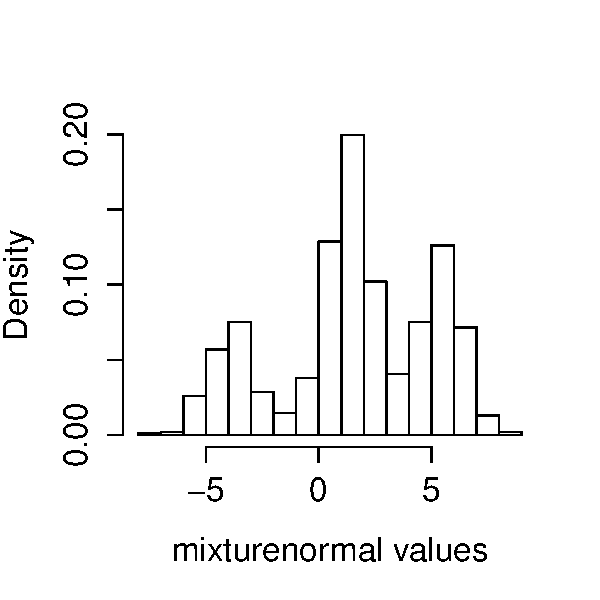
\includegraphics[scale=0.75]{Histogram.pdf}
\caption{Histogram of the mixturenormal data suggesting that the data is in fact a mixture of three separate Normal distributions.}
\label{F:Box}
\end{center}
\end{figure}

The E-M algorithm was used to estimate the mean and weight of each distribution. The missing data are the class labels, $z_i$, identifying which of the $K$ distributions each observation belongs to. Because the data are a mixture of normal distributions the simplified form of the E-M algorithm based on sufficient statistics (S= ($\sum Z_i$, $\sum_{z_i=1} X_i$, $\sum_{z_i=2} X_i$, $\sum_{z_i=3} X_i$ )) was used. The density function of a mixture Normal distribution with unit variance is a weighted sum of the $K$ component Normal distributions as follows:

\[
f(x)= \sum_{k=1}^K\phi_k \frac{1}{2\pi}\exp\{\frac{-(x-\mu_k)^2}{2}  \}
\]

Therefore the following parameters had to be estimated for each of the 3 distributions:

$\mu_k$: the mean of the k\textsuperscript{th} normal distribution
 
$\phi_k$: the weight or proportion of the total data lying in  k\textsuperscript{th} normal distribution


%The missing data was taken to be the class labels for each point identifying which of the three distributions each point belonged to. If this information was provided then the Maximim Likelihood Estimates could have been used to estimate the weights and means.
 
During the E-step the likelihood of each point being a member of the k\textsuperscript{th} distribution is computed as follows:

\[
f(x,z|\phi, \mu)= \frac{\phi_k \frac{1}{2\pi}\exp\{\frac{-(x-\mu_k)^2}{2}  \}}{ \sum_{k=1}^K\phi_k \frac{1}{2\pi}\exp\{\frac{-(x-\mu_k)^2}{2}  \}}
\]
 
 During the M-Step the parameters are updated as follows:

\[
\phi_{new_k} = \frac{\sum_{i=1}^n f(x,z|\phi_{old_k}, \mu_{old_k})}{n}
\]

\[
\mu_{new_k} = \frac{\sum_{i=1}^n f(x,z|\phi_{old_k}, \mu_{old_k})x_i}{\sum_{i=1}^n f(x,z|\phi_{old_k}, \mu_{old_k})}
\]

where: n = number of observations and K = 3.
 
The model was run iteratively until the parameter estimates had converged. The R code used is given in Appendix 1.

\subsection{Results}

\begin{table}[ht]
\begin{center}
\begin{tabular}{llllll}
  \hline
 $\mu_1$ &  $\mu_2$ & $\mu_3$ & $\phi_1$ & $\phi_2$ & $\phi_3$\\ 
  \hline
-3.89 & 1.32 & 5.46 & 0.20 & 0.49 & 0.31 \\
  \hline
\end{tabular}
\caption{The estimated means and weights of each of the 3 component distributions (rounded to 2 decimal places).} 
\label{T:Times}
\end{center}
\end{table}

The model was run 1000 times using a range of initial estimates (drawn randomly from the parameter space) for each of the parameters. In all cases the model converged on a single estimate indicating that it was robust to choice of starting values however the number iterations required to converge varied but was generally less than 40 iterations. The model converged after 32 iterations when initial values based on visual estimation of the three modes and equal weight given to each distribution was used. The estimated means and weights of the three normal distributions are given in Table 1. Figure 2 shows a histogram of the data overlain with the density function based on the maximum likelihood estimates of the parameters. The three modes in the density function are reasonably aligned with the three modes in the histogram suggesting that the model has accurately estimated the unknown parameters. The estimates of the weights also appear consistent with the relative sizes of the three distributions.

\begin{figure}[h]
\begin{center}
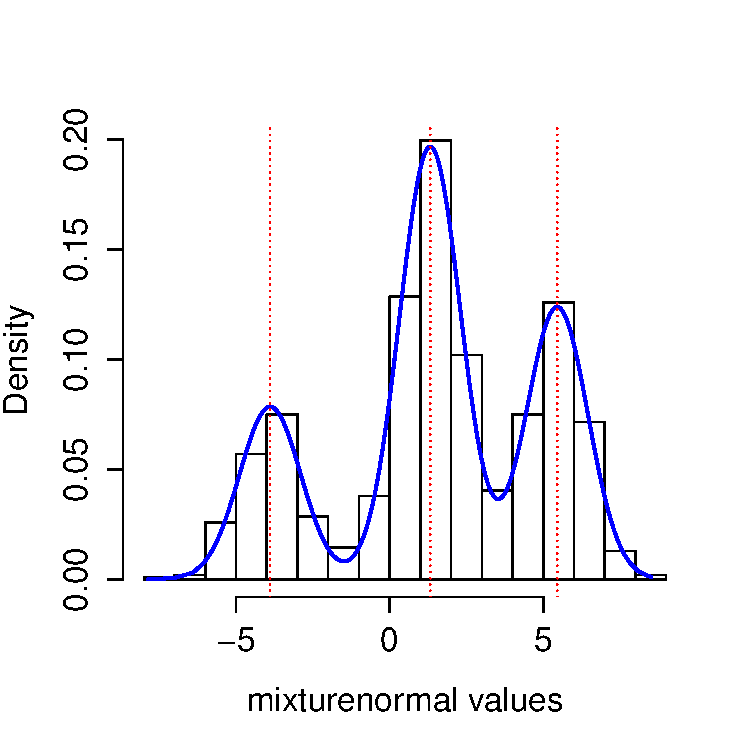
\includegraphics[scale=0.75]{density.pdf}
\caption{Histogram of the mixturenormal data overlain with the density function based on the maximum likelihood estimates of the unknown parameters.}
\label{F:Box}
\end{center}
\end{figure}

\section{Solution 2: Variance Test}
\begin{figure}[h]
\begin{center}
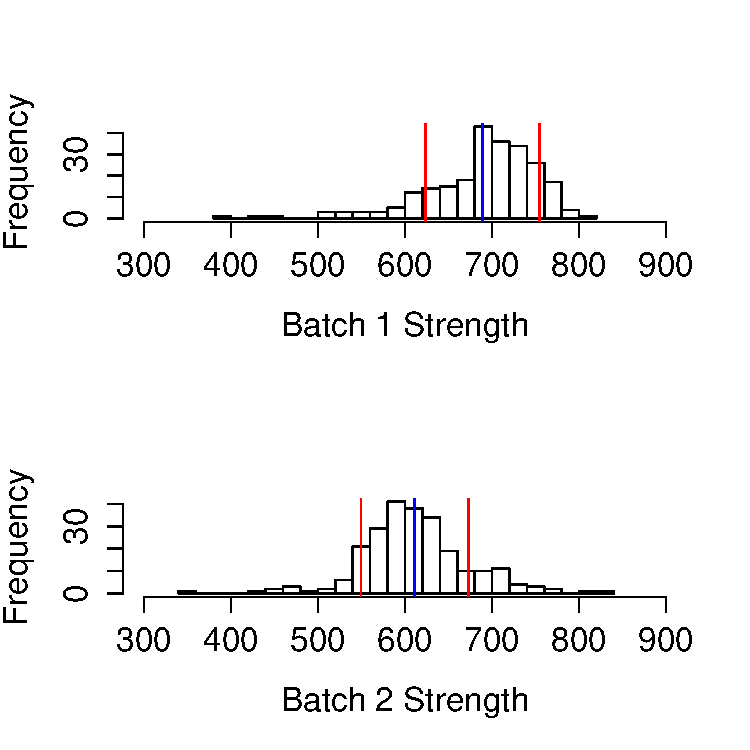
\includegraphics[scale=0.75]{batchHist.pdf}
\caption{Histograms of the strengths (units not supplied) of batch 1 (top) and batch 2 (bottom). The blue line shows the mean while the red lines show the standard deviation. The sample variance of ceramic strength of batch 1 is larger than that of batch 2.}
\label{F:Box}
\end{center}
\end{figure}

The histograms in Figure 3 show that ceramic strength of both batches have non-Normal distributions with batch 1 skewed to the right and batch 2 being symmetric but heavy tailed. This suggests that a standard F test to compare the variances might not be robust and that an alternative bootstrap based test is preferable. Both batches have 240 observations and are hence reasonably sized for bootstrapping. Non-parametric bootstrapping was used to from the empirical CDF of the test statistic. The test statistic used to assess the equality of variances of the two batches is the ratio of the batch variances is:

\[
T =\frac{var(batch 1)}{var(batch 2)}
\]

where
\[
T_{obs} \approx 1.12
\]

If the batches have the same variances then the ratio should equal 1. If batch 1 has greater or lesser variance than batch 2 then the ratio will be greater then or less than 1 accordingly. The observed value of the test statistic is approximately 1.12 suggesting that variance of the ceramic strength of batch 1 is greater than that of batch 2, however this could be a chance effect of sampling. The hypothesis under test is as follows:

\[
H_0 =\frac{var(batch 1)}{var(batch 2)} = 1
\]
\[
H_1 =\frac{var(batch 1)}{var(batch 2)} \neq 1
\]

During bootstrapping the batches were not pooled, each batch was sampled with replacement separately. 100000 iterations were used. The R code is given in Appendix 2.

\begin{figure}[H]
\begin{center}
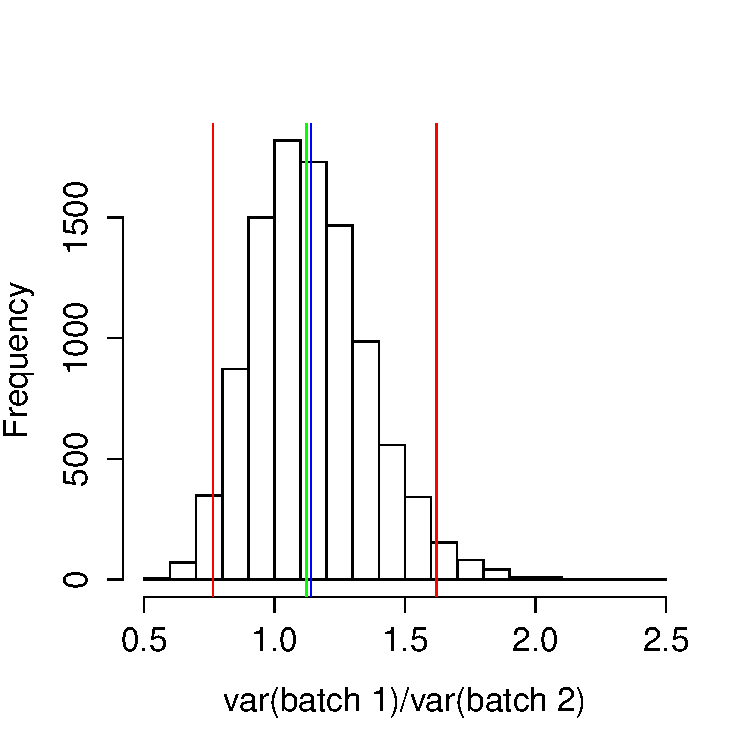
\includegraphics[scale=0.75]{cdf.pdf}
\caption{The bootstrap distribution of the test statistic. The green line shows the observed value while blue line shows the mean and the red lines show the 95\% confidence interval. 100000 iterations were used during the bootstrap.}
\label{F:Box}
\end{center}
\end{figure}

The empirical distribution of the test statistic is shown in Figure 4. The observed test statistic is close to the mean suggesting that bias is not an issue. The 95\% confidence interval (estimated using the relevant percentiles) of the bootstrapped ratio of the variances is approximately 0.76 to 1.63. While there appears to be considerable variability in the strength of the ceramic materials, the 95\% confidence interval contains 1 hence at this level there is no evidence to suggest that the ceramic strengths of the two batches are different. A study based on a larger sample size or investigating additional variables might explain the observed variation in ceramic strength.



\clearpage
\appendix
\section{Appendix}

\subsection{ }
Implementation of the E-M algorithm for a 1D  mixture Normal distribution in R where the variance of each component distribution is 1.

\begin{verbatim}
x <- dget("mixturenormal.txt")

# x is the data
# mu are the initial estimate of the means
# phi are the initial estimates of the weights
em <- function(x, mu, phi, maxIterations=1000)
{
  #save the initial estimates for monitoring the results
  initialMu <- mu
  initialPhi <- phi
  #K, the number of component distributions
  numberOfDistributions <- length(mu)
  densityK <- matrix(nrow=length(x), ncol=length(mu),byrow=T)
  densityAll <- rep(0, length(x))
  converged <- FALSE
  #variables used for monitoring convergence
  i <- 0
  prevMu <- rep(0, numberOfDistributions)
  prevPhi <- rep(0, numberOfDistributions)
  
  #continue until all parameter estimates have converged
  while(!converged)
  {
    i <- i+1
    #E-Step: calulate the likelihood that each point belongs to each distribution 
    densityAll <- rep(0, length(x))
    for(k in 1:numberOfDistributions)
    {
      densityAll <- densityAll + (dnorm(x, mu[k], 1)*phi[k])
    }
    
    for(k in 1:numberOfDistributions)
    {
      densityK[,k] <- (dnorm(x, mu[k], 1)*phi[k])/densityAll
    }
    
    #M-Step: use the likelihood to update the parameter estimates
    for(k in 1:numberOfDistributions)
    {
      mu[k] <- sum(densityK[,k]*x)/sum(densityK[,k])  
      phi[k] <- sum(densityK[,k])/length(x)
    }
    
    #check if all parameters have converged or the max iterations has been reached
    converged <- (mu - prevMu <10^-10) && (phi - prevPhi == 0)
    if (i > maxIterations)
    {
      converged = T
      message("Exiting as parameters are converging to slowly: diff mu = ", mu - prevMu, 
       " diff phi = ", phi - prevPhi)
    }
    prevMu <- mu
    prevPhi <- phi
  }
  list("densityAll"=densityAll, "densityK"=densityK, "mu"=mu, "phi"=phi, "iterations"=i,
   "initialMu"= initialMu, "initialPhi"=initialPhi)
}

#run multiple times using random initial values
n <- 1000
results <- matrix(nrow=n, ncol=13,byrow=T)
colnames(results) <- c("initial mu1", "initial mu2", "initial mu3", "initial phi1",
 "initial phi2", "initial phi3","mu1", "mu2", "mu3", "phi1", "phi2", "phi3", "iterations")
for (m in 1:n)
{
  res <- em(x,mu=runif(3, min(x), max(x)),phi=runif(3))
  results[m,1:3] <- (res$initialMu)
  results[m,4:6] <- (res$initialPhi)
  results[m,7:9] <- (res$mu)
  results[m,10:12] <- (res$phi)
  results[m,13] <- res$iterations
}

#initial estimates of mean from visual inspection of histogram
mu <- c(-3, 2, 5) # the mean
phi <- c(1/3,1/3,1/3) # the weight of each distribution
emResults <- em(x,mu,phi)

#plot the histogram with density function and parameter estimates
hist(x, prob=TRUE, main="", xlab="mixturenormal values")
lines(smooth.spline(x, emResults$densityAl, spar=0.35), col="blue", lwd=2)
abline(v=emResults$mu, lty="dotted", col="red")

\end{verbatim}


\subsection{ }

R code to form the empirical distribution of the test statistic to test equality of variance of the ceramic strength of the two batches.

\begin{verbatim}
data <- read.csv("ceramic.csv")
b1 <- data[data$batch==1,]$strength
b2 <- data[data$batch==2,]$strength

varRatio <- function(x1, x2) { var(x1)/var(x2)}
twoSampleVarTest <- function(x1, x2, n, test)
{
  Tobs = test(x1, x2)
  ratios = rep(NA, n)
  for (i in 1:n)
  {
    x1n <- sample(x1, length(x1), replace=T)
    x2n <- sample(x2, length(x2), replace=T)
    ratios[i] <- test(x1n, x2n)
  } 
  hist(ratios, xlab="var(batch 1)/var(batch 2)", main="",nclass=19)
  abline(v=Tobs, col='green')
  abline(v=mean(ratios), col='blue')
  cis <- quantile(ratios, c(0.025, 0.975))  
  abline(v=cis, col='red')
  list("CI"=cis, "Tobs"=Tobs)
}

twoSampleVarTest(b1, b2, 100000, varRatio)

\end{verbatim}
\label{S:A1}


\end{document}

